\documentclass[a4paper,11pt]{report}
\usepackage{chuan_math_gkt}
\usetikzlibrary{angles,quotes,intersections,patterns,decorations.pathreplacing}
\chuanexamsetup

\begin{document}
\examfontsize

\examsecret{绝密$\bigstar$启用前}

\examtitle{2023年普通高等学校招生全国统一考试（新课标I卷）}{数\quad 学}

\noticetitle
\begin{examnotice}
\item 答卷前，考生务必将自己的姓名、准考证号填写在答题卡上. 
\item 回答选择题时，选出每小题的答案后，用铅笔把答题卡上对应题目的答案标号涂黑. 如需改动，用橡皮擦干净后，再选涂其他答案标号. 回答非选择题时，将答案写在答题卡上. 写在本试卷上无效. 
\item 考试结束后，将本试卷和答题卡一并交回. 
\end{examnotice}

\examsection{一、选择题：本题共8小题，每小题5分，共40分. 在每小题给出的四个选项中，只有一项是符合题目要求的. }
\begin{examquestions}
\item 已知集合$M=\{-2,-1,0,1,2\}$，$N=\{x\mid x^2-x-6\geq0\}$，则$M\cap N=$
\fourchoices{$\{-2,-1,0,1\}$}{$\{0,1,2\}$}{$\{-2\}$}{$2$}
\item 已知$z=\dfrac{1-\mathrm{i}}{2+2\mathrm{i}}$，则$z-\overline z=$
\fourchoices{$-\mathrm{i}$}{$\mathrm{i}$}{$0$}{$1$}
\item 已知向量$\vec a=(1,1)$，$\vec b=(1,-1)$，若$(\vec a+\lambda\vec b)\perp(\vec a+\mu\vec b)$，则
\twochoices{$\lambda+\mu=1$}{$\lambda+\mu=-1$}{$\lambda\mu=1$}{$\lambda\mu=-1$}
\item 设函数$f(x)=2^{x(x-a)}$在区间$(0,1)$上单调递减，则$a$的取值范围是
\twochoices{$(-\infty,-2]$}{$[-2,0)$}{$(0,2]$}{$[2,+\infty)$}
\item 设椭圆$C_1:\dfrac{x^2}{a^2}+y^2=1(a>1)$，$C_2:\dfrac{x^2}{4}+y^2=1$的离心率分别为$e_1,e_2$. 若$e_2=\sqrt3e_1$，则$a=$
\fourchoices{\tallchoice{$\dfrac{2\sqrt3}{3}$}}{$\sqrt2$}{$\sqrt3$}{$\sqrt6$}
\item 过点$(0,-2)$与圆$x^2+y^2-4x-1=0$相切两条直线的夹角为$\alpha$，则$\sin\alpha=$
\fourchoices{$1$}{\tallchoice{$\dfrac{\sqrt{15}}4$}}{\tallchoice{$\dfrac{\sqrt{10}}4$}}{\tallchoice{$\dfrac{\sqrt6}4$}}
\item 记$S_n$为数列$\{a_n\}$的前$n$项和，设甲：$\{a_n\}$为等差数列；乙：$\left\{\dfrac{S_n}{n}\right\}$为等差数列，则
\onechoices{甲是乙的充分条件但不是必要条件}{甲是乙的必要条件但不是充分条件}{甲是乙的充要条件}{甲既不是乙的充分条件也不是乙的必要条件}
\item 已知$\sin(\alpha-\beta)=\dfrac13$，$\cos\alpha\sin\beta=\dfrac16$，则$\cos(2\alpha+2\beta)=$
\fourchoices{\tallchoice{$\dfrac79$}}{\tallchoice{$\dfrac19$}}{\tallchoice{$-\dfrac19$}}{\tallchoice{$-\dfrac79$}}
\end{examquestions}

\examsection{二、选择题：本题共4小题，每小题5分，共20分. 在每小题给出的选项中，有多项符合题目要求. 全部选对的得5分，部分选对的得2分，有选错的得0分. }
\begin{examquestions}[start=9]
\item 有一组样本数据$x_1,x_2,\cdots,x_6$，其中$x_1$是最小值，$x_6$是最大值，则
\onechoices{$x_2,x_3,x_4,x_5$的平均数等于$x_1,x_2,\cdots,x_6$的平均数}{$x_2,x_3,x_4,x_5$的中位数等于$x_1,x_2,\cdots,x_6$的中位数}{$x_2,x_3,x_4,x_5$的标准差不小于$x_1,x_2,\cdots,x_6$的标准差}{$x_2,x_3,x_4,x_5$的极差不大于$x_1,x_2,\cdots,x_6$的极差}
\item 噪声污染问题越来越受到重视. 用声压级来度量声音的强弱，定义声压级$L_p=20\lg\dfrac{p}{p_0}$，其中常数$p_0(p_0>0)$是听觉下限阈值，$p$是实际声压. 下表为不同声源的声压级：
\begin{tightcenter}\begin{tabular}{|c|c|c|}\hline 声源&与声源的距离/m&声压级/dB\\\hline 燃油汽车&10&$60\sim90$\\\hline 混合动力汽车&10&$50\sim60$\\\hline 电动汽车&10&40\\\hline\end{tabular}\end{tightcenter}
已知在距离燃油汽车、混合动力汽车、电动汽车$10$m处测得实际声压分别为$p_1,p_2,p_3$，则
\twochoices{$p_1\geq p_2$}{$p_2>10p_3$}{$p_3=100p_0$}{$p_1\leq100p_2$}
\item 已知函数$f(x)$定义域为$\mathbb R$，$f(xy)=y^2f(x)+x^2f(y)$，则
\twochoices{$f(0)=0$}{$f(1)=0$}{$f(x)$是偶函数}{$x=0$为$f(x)$的极小值点}
\item 下列物体中，能够被整体放入棱长为$1$（单位：m）的正方体容器（容器壁厚度忽略不计）内的有
\onechoices{直径为$0.99$m的球体}{所有棱长均为$1.4$m的四面体}{底面直径为$0.01$m，高为$1.8$m的圆柱体}{底面直径为$1.2$m，高为$0.01$m的圆柱体}
\end{examquestions}

\examsection{三、填空题：本题共4小题，每小题5分，共20分. }
\begin{examquestions}[start=13]
\item 某学校开设了$4$门体育类选修课和$4$门艺术类选修课，学生需从这$8$门课中选修$2$门或$3$门课，并且每类选修课至少选修$1$门，则不同的选课方案共有\blank 种（用数字作答）. 
\item 在正四棱台$ABCD-A_1B_1C_1D_1$中，$AB=2$，$A_1B_1=1$，$AA_1=\sqrt2$，则该棱台的体积为\blank. 
\item 已知函数$f(x)=\cos\omega x-1(\omega>0)$在区间$[0,2\pi]$有且仅有$3$个零点，则$\omega$的取值范围是\blank. 
\item 已知双曲线$C:\dfrac{x^2}{a^2}-\dfrac{y^2}{b^2}=1(a>0,b>0)$的左、右焦点分别为$F_1,F_2$. 点$A$在$C$上，点$B$在$y$轴上，$F_1A\perp F_1B$，$F_2A=-\dfrac23F_2B$，则$C$的离心率为\blank. 
\end{examquestions}

\examsection{四、解答题：本题共6小题，共70分. 解答应写出文字说明、证明过程或演算步骤. }
\begin{examanswers}[start=17]
\item（10分）

已知在$\triangle ABC$中，$A+B=3C$，$2\sin(A-C)=\sin B$. 

\subq{（1）}{求$\sin A$；}

\subq{（2）}{设$AB=5$，求$AB$边上的高.}

\item（12分）

如图，在正四棱柱$ABCD-A_1B_1C_1D_1$中，$AB=2$，$AA_1=4$. 点$A_2,B_2,C_2,D_2$分别在棱$AA_1,BB_1,CC_1,DD_1$上，$AA_2=1$，$BB_2=DD_2=2$，$CC_2=3$. 

\noindent\begin{minipage}[t]{0.64\linewidth}
\subq{（1）}{证明：$B_2C_2\parallel A_2D_2$；}

\subq{（2）}{点$P$在棱$BB_1$上，当二面角$P-A_2C_2-D_2$为$150^\circ$时，求$B_2P$.}
\end{minipage}\hfill
\begin{minipage}[t]{0.2\linewidth}
\vspace{-1.8em}
\centering
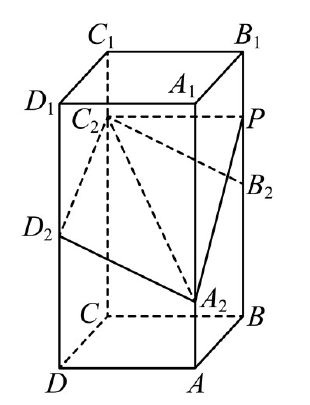
\includegraphics[width=\linewidth]{figures/2023_xgk1_q18.png}
\end{minipage}

\item（12分）

已知函数$f(x)=a(e^x+a)-x$. 

\subq{（1）}{讨论$f(x)$的单调性；}

\subq{（2）}{证明：当$a>0$时，$f(x)>2\ln a+\dfrac32$.}

\item（12分）

设等差数列$\{a_n\}$的公差为$d$，且$d>1$. 令$b_n=\dfrac{n^2+n}{a_n}$，记$S_n,T_n$分别为数列$\{a_n\}$，$\{b_n\}$的前$n$项和. 

\subq{（1）}{若$3a_2=3a_1+a_3$，$S_3+T_3=21$，求$\{a_n\}$的通项公式；}

\subq{（2）}{若$\{b_n\}$为等差数列，且$S_{99}-T_{99}=99$，求$d$.}

\item（12分）

甲、乙两人投篮，每次由其中一人投篮，规则如下：若命中则此人继续投篮，若未命中则换为对方投篮. 无论之前投篮情况如何，甲每次投篮的命中率均为$0.6$，乙每次投篮的命中率均为$0.8$. 由抽签确定第$1$次投篮的人选，第$1$次投篮的人是甲、乙的概率各为$0.5$. 

\subq{（1）}{求第$2$次投篮的人是乙的概率；}

\subq{（2）}{求第$i$次投篮的人是甲的概率；}

\subq{（3）}{已知：若随机变量$X_i$服从两点分布，且$P(X_i=1)=1-P(X_i=0)=q_i$，$i=1,2,\cdots,n$，则$E\left(\sum_{i=1}^n X_i\right)=\sum_{i=1}^n q_i$. 记前$n$次（即从第$1$次到第$n$次投篮）中甲投篮的次数为$Y$，求$E(Y)$.}

\item（12分）

在直角坐标系$xOy$中，点$P$到$x$轴的距离等于点$P$到点$\left(0,\dfrac12\right)$的距离，记动点$P$的轨迹为$W$. 

\subq{（1）}{求$W$的方程；}

\subq{（2）}{已知矩形$ABCD$有三个顶点在$W$上，证明：矩形$ABCD$的周长大于$3\sqrt3$.}
\end{examanswers}

\end{document}
